\documentclass[12pt]{article}% uses letterpaper by default

%---------- Uncomment one of them ------------------------------
\usepackage[includeheadfoot, top=1in, bottom=1in, hmargin=1in]{geometry}

% \usepackage[a5paper, landscape, twocolumn, twoside,
%    left=2cm, hmarginratio=2:1, includemp, marginparwidth=43pt, 
%    bottom=1cm, foot=.7cm, includefoot, textheight=11cm, heightrounded,
%    columnsep=1cm, dvips,  verbose]{geometry}
%---------------------------------------------------------------
\usepackage{fancyhdr}
\renewcommand{\footrulewidth}{0.4pt}% default is 0pt
\usepackage{verbatim}
\usepackage{url}
\usepackage{cancel}
\pagestyle{fancy}
\usepackage{graphicx}
\usepackage{setspace}
\singlespacing
%\doublespacing
%\onehalfspacing
%\newcommand{\exercisename}{}
\usepackage{varwidth}

\newcommand{\degrees}{\ensuremath{^\circ}}
\newcommand{\arcmin}{\ensuremath{'}}
\newcommand{\arcsec}{\ensuremath{"}}
\newcommand{\hours}{\ensuremath{^\mathrm{h}}}
\newcommand{\minutes}{\ensuremath{^\mathrm{m}}}
\newcommand{\seconds}{\ensuremath{^\mathrm{s}}}

\newcommand{\s}[0]{\phantom{i}} %sets up \s command
\newcommand{\m}[0]{\phantom{abcde}} %sets up \m command
\providecommand{\e}[1]{\ensuremath{\times 10^{#1}}} %sets up \e command
\setlength{\parindent}{0.2in} %new paragraph indent
\usepackage{indentfirst} % indent the first paragraph of a section
\usepackage{amsmath}
\usepackage{enumitem}

\lhead{Astronomy Lab I}
\rhead{Fall 2021}
\cfoot{\thepage}


\begin{document}

\begin{center}
    \LARGE Lab 7: Exoplanet Detection
\end{center}

\section{Introduction}

In the past 20 years or so, the field of extrasolar planet (exoplanet) astronomy has exploded. 
The first exoplanet was detected in 1992, and as of October 22, 2021, we know of 4538 confirmed exoplanets\footnote{\url{http://exoplanetarchive.ipac.caltech.edu/}}. In this lab we'll explore how exoplanets are actually detected and try to understand the advantages and disadvantages of different detection methods. 
\begin{itemize}
    \item Write a sentence or two in your lab notebook briefly explaining how you might go about detecting a planet around another star. 
\end{itemize}

\section{Detection Methods}

\subsection{Radial Velocity} 

\vspace{0.1in}

\noindent With the radial velocity method, planets are detected based on their gravitational pull on the host star. This pull causes the star to move as the planet orbits. We can detect the star's motion (and infer the planet's presence) because the wavelength (i.e., color) of the starlight received at Earth changes as the star moves due to the \textit{Doppler effect.}  \\

\noindent Let's look at \textbf{Newton's law of gravity}.  Newton's law of gravity states that the gravitational force between two objects is related to the mass of the two objects and the distance between them.  We have:

\begin{equation}
F_{gravity}  = G \frac{M m}{r^2}
\end{equation}

\noindent where $G$ is the universal constant of gravitation ($6.67$x$10^{-11} \frac{m^3}{kg s^2}$), $M$ and $m$ are the masses of the two objects attracting each other, and $r$ is the distance between their centers of mass. For a planet orbiting around a star, $M$ is the mass of the star, $m$ is the mass of the planet, and $r$ is the distance between the planet and the star. 

\begin{enumerate}
    \item What variables are important in measuring radial velocities? What variables aren't? 
    \item For each important variable, describe what increasing and decreasing it does to the observed radial velocity.
\end{enumerate}

\subsection{Transits}

The transit method is a bit easier to understand. When a planet passes in front of a star, it blocks some of that star's light from reaching the Earth. So, if you observe that star multiple times and notice a periodic dip in the flux of photons, you can conclude that a planet is rotating around the star.
\begin{enumerate}
    \item What variables are important here that were unimportant in the radial velocity method, and vice versa?
    \item For each important variable, describe what increasing and decreasing it does to the observed transit. 
\end{enumerate}

\subsection{Kepler's Third Law}

Kepler's third law of planetary motion tells us that the square of the orbital period ($P$) of a planet is proportional to the cube of the semimajor axis ($a$) of its orbit, or:
\begin{equation*}
P^2 \propto a^3.
\end{equation*}
\begin{enumerate}
    \item Would it be easier to detect exoplanets with short or long orbital periods via the transit method? 
    What about the radial velocity method? 
    \item Is the transit method more sensitive to exoplanets with small or large semimajor axes? 
    What about the radial velocity method? Make sure you explain your answers.
\end{enumerate}


\section{Observations of Exoplanets} 

We will be using an online applet to help us understand the observations of varying star-planet systems.  
Go to the following website: \url{https://astro.unl.edu/nativeapps/} and install NAAP Labs software. 
Open the application on your computer and  first click on the ``Extrasolar Planets" and then on the ``Exoplanet Radial Velocity Simulator" link. Familiarize yourself with the layout and the various parameters you can manipulate.

\subsection{Exoplanet Radial Velocity Simulator}

\begin{enumerate}
\item Select ``Option A''' in the \textit{Presets} box, and click ``set''. 
List the default properties of the star and planet.  What is the period of the system?
\item A plot of the radial velocity of the star is shown in the upper right.  Be sure that there is a check mark next to ``show theoretical curve'' and ``show simulated measurements.''  
Why don't the measurements lie exactly on the theoretical curve?
\item Use the slider to decrease the noise of the observations.  
Describe what happens. Why is the unit of the noise in m/s?
\item Reset the noise to 15 m/s. In the \textit{Planet Properties} box move the ``mass'' slider to change the mass of the planet.  Describe what happens and why.
\item In the \textit{Planet Properties} box move the ``semimajor axis'' slider to change the semimajor axis of the planet's orbit.  
Describe what happens and why.
\item In the \textit{Planet Properties} box move the ``eccentricity'' slider to change the eccentricity of the planet's orbit.  Describe the changes you see in the diagram on the left and the plot on the right. Why does the radial velocity plot become asymmetric?
\item The mass of Earth is equivalent to approximately 0.003 Jupiter masses.  
Use the simulator to determine if we could detect an ``Earth'' around another star using the radial velocity method.
\end{enumerate}

\subsection{Exoplanet Transit Simulator}

Go back in your web browser and click on ``Exoplanet Transit Simulator.'' 
You can use the phase slider (bottom right) to show where the planet is at various points along the light curve.  
Note that the light curve does not show a full orbit of the planet, but only the part right around its transit.

\begin{enumerate}
\item Select ``Option A'' in the \textit{Presets} box, and click ``set.''  Set the noise to $\approx 0.001$ (you may want to type it into the box and hit enter).  
List the default properties of the star and planet. 
\item In the \textit{Planet Properties} box move the ``mass'' slider to change the mass of the planet. Describe what happens to the plot of normalized flux and why.
\item In the \textit{Planet Properties} box move the ``radius'' slider to change the radius of the planet. Describe what happens to the plot of normalized flux and why.
\item In the \textit{Star Properties} box move the ``mass'' slider to change the mass of the host star. Describe what happens to the plot of normalized flux and why.
\item Use the \textit{System Orientation and Phase} box to determine the range of inclinations within which this planet could be detected via the transit method.  
You may need to type numbers into the box, the slider is hard to move in small or consistent increments.
\item In the \textit{Presets} box select a different option.  
List the parameters of this option and describe the normalized flux curve.  
How is the curve different from Option A and why?
\end{enumerate}


\section{Exoplanet Characteristics}

Now we will be using an online applet that allows us to plot characteristics of detected exoplanets. Go to the following website: \url{http://exoplanets.org}.  
Click on the big button that says \textit{Plots} on in the middle.  
To start your first plot, click on \textit{Scatter Plot}. There are three options that you will be experimenting with.  
\textit{Filter} allows you to plot only exoplanets that were detected with a certain method.  
And \textit{x} and \textit{y} allow you to change which quantities will be plotted on the x-axis and y-axis.

\begin{enumerate}
\item Plot orbital period on the y-axis vs. mass ($m \sin(i)$ gives the minimum mass of the planet) on the x-axis.  
What is the range of mass and orbital period?  (Be sure to include units, and watch out for log vs. linear axes!)  
What masses and orbital periods do most exoplanets have?
\item Now click ``Add Filter'', and select ``RV Planets'' from the dropdown ``filter'' menu so that only exoplanets detected via the radial velocity method are shown.  
Does the plot change? If so, how?  
\item Change the Filter option to ``Transit Planets.'' 
Explain the differences that you see and explain why this is the case based on what you know about the sensitivities of the two detection methods.
\item Change the Filter option back to ``No Filter.'' 
Now plot semimajor axis vs. mass. Explain what you see.
\item Again, select only ``RV Planets'' and then only ``Transits.''
Account for the differences between the two plots.
\item Now plot only ``Hot Jupiters.''  Note the range of the x-axis and y-axis. 
Why do you think these exoplanets are called ``hot Jupiters?"
\end{enumerate}

\section{Detect exoplanets with TESS (optional but fun!)}

If there's time left in the lab, you will help discover new exoplanets. Transiting Exoplanet Survey Satellite (TESS) surveys two-hundred-thousand stars, measuring their brightness as a function of time. With lots of new data coming in fast, you can help the research team discover new exoplanets by marking the exoplanet candidates in their data. Start by going to the website: https://www.zooniverse.org/projects/nora-dot-eisner/planet-hunters-tess. Review the transit method about which we just learned in lab, and follow the instructions in the tutorial of the ``Classify Tab." Register and start classifying! 

\section{Conclusions}
\begin{figure}
    \centering
    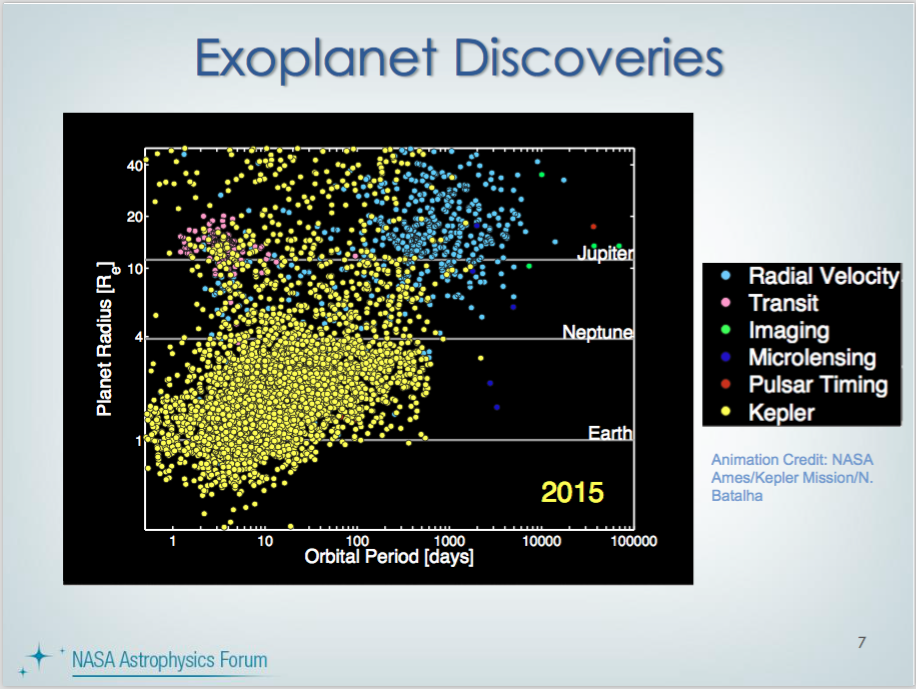
\includegraphics[width=\textwidth]{Batalha_plot.png}
    \caption{Ecoplanet Discoveries}
    \label{fig:my_label}
\end{figure}
\begin{enumerate}
\item Now that you've played around with some interactive demos, explain the radial velocity exoplanet detection method in your own words (2-4 sentences).
\item Explain the transit exoplanet detection method in your own words (2-4 sentences).
\item Based on the supplemental plot, what method did the 
\item Some regions in the ``Exoplanet Discoveries'' plot do not have any objects in them. 
Based on what you know about the sensitivities of various detection methods, do you think those empty regions are characteristic of the population of exoplanets or a selection effect? Why?
\item What was the most interesting thing you learned today?
\item Ask a question.
\end{enumerate}

\end{document}